\documentclass{article}
\usepackage[a4paper, margin=0.5in]{geometry}
\usepackage{fontspec}
\usepackage{fontsize}
\usepackage{enumitem}
\usepackage{graphicx}
\usepackage{wrapfig}
\usepackage{xcolor}
\usepackage[breakable, skins]{tcolorbox} % Corrected tcolorbox inclusion
\usepackage{array}
\usepackage{tabularx}
\usepackage{booktabs}
\usepackage{float}
\usepackage{adjustbox} % Include the package
\usepackage{pdflscape}
\usepackage{fancyhdr} % Added fancyhdr package

\setmainfont{Roboto}

\pagestyle{fancy}
\fancyhf{}
\fancyfoot[C]{\thepage}
\renewcommand{\headrulewidth}{0pt}

\pagestyle{empty} % Remove all headers and footers

\begin{document}
\tcbset{
    width=\textwidth, % Ensures all tcolorboxes have full text width
    colback=gray!20, % Background color (adjust if needed)
    colframe=black, % Border color
    boxrule=0.5pt, % Border thickness
}
\fontsize{14}{20}\selectfont

\begin{center}
    \fontsize{18}{22}\selectfont
    \textbf{Music Expectations}
\end{center}

\vspace{2em}

\noindent When learning at Colchester Academy, you should follow these rules:

\vspace{2em}

\noindent\textbf{Be prepared}
\vspace{0.5em}

\par \noindent Make sure that you start any tasks straight away
\par \noindent Always have the correct equipment.

\vspace{3em}

\noindent\textbf{Be polite}
\vspace{0.5em}

\par \noindent  Raise your hand to speak to the teacher.
\par \noindent  Make sure that you stay in your seat, unless given permission to move.
\par \noindent  Listen to others when performing, and give constructive feedback.

\vspace{3em}

\noindent\textbf{Look after one another}
\vspace{0.5em}
\par \noindent  Make sure all cables are tidy, and headphones are looked after.
\par \noindent  Move around the room quietly and purposefully.\
\par \noindent  Use mini-whiteboards only when asked to.
\par \noindent  Pack any resources away with care.
\newpage

\begin{center}
    \fontsize{18}{22}\selectfont
    \textbf{What will I learn this half-term?}
\end{center}

\vspace{1em}

\noindent This half-term I will be introduced to instruments of the orchestra. If I can listen to music from an orchestra, I will learn about a lot of different sounds and styles of music.
I will learn about Dvorak’s New World Symphony, which is a famous piece of music for an orchestra.


\vspace{1em}

\noindent It’s important to learn this piece because:

\vspace{2.5em}

\begin{itemize}[leftmargin=0em, itemsep=0pt, parsep=0pt, topsep=0pt]
    \item Through listening and playing, I’ll be able to identify more instruments as I listen to them.

    \item It will help me listen to other styles of music and enjoy them more.
\end{itemize}

\vspace{2.5em}
\par \noindent
I should still use the correct fingers, and I should be able to play my piece of music with confidence, as long as I practise hard and do not give up.

\vspace{2.5em}

\noindent Each lesson I will be expected to work hard and participate.\

\vspace{2.5em}

\noindent If I have a question, I will put my hand up.

\vspace{1em}
\noindent When working on the keyboards, I will work quietly.

\vspace{1em}
\noindent I will start every lesson with the Do Now, which is to be completed in silence.


\newpage
\begin{center}
    \fontsize{18}{22}\selectfont
    \textbf{Task 1 - Families Of The Orchestra}
\end{center}

\vspace{1em}

\setlength{\columnsep}{1.5em}

\noindent
All of these instruments belong to either:
\vspace{1em}
\par \noindent Brass
\par \noindent Woodwind
\par \noindent Strings
\par \noindent Percussion

\vspace{1em}



\vspace{2em}

\begin{minipage}[t]{0.48\textwidth}
    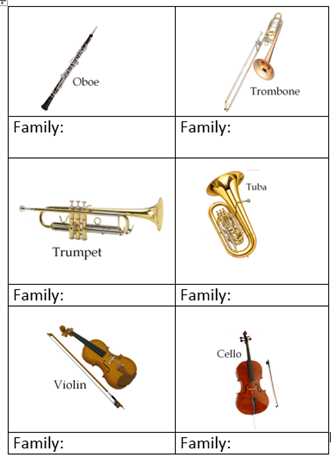
\includegraphics[width=\linewidth]{fam1.png}
\end{minipage}
\hfill
\begin{minipage}[t]{0.48\textwidth}
    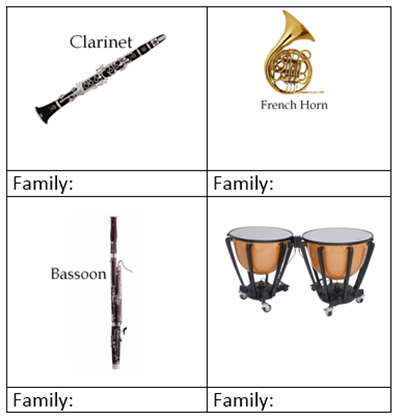
\includegraphics[width=\linewidth]{fam2.png}
\end{minipage}

\vspace{2em}

\noindent Write the correct family name for each instrument. 
\par \noindent Look at the posters on the wall to help you.


\newpage

\begin{center}
    \fontsize{18}{22}\selectfont
    \textbf{Task 2 - ‘Star Wars’ theme by John Williams}
\end{center}

\vspace{1em}

\setlength{\columnsep}{1.5em} % Adjust spacing between text and image

\begin{wrapfigure}{l}{0.3\linewidth} 
    \vspace{-0.8em} 
    \centering
    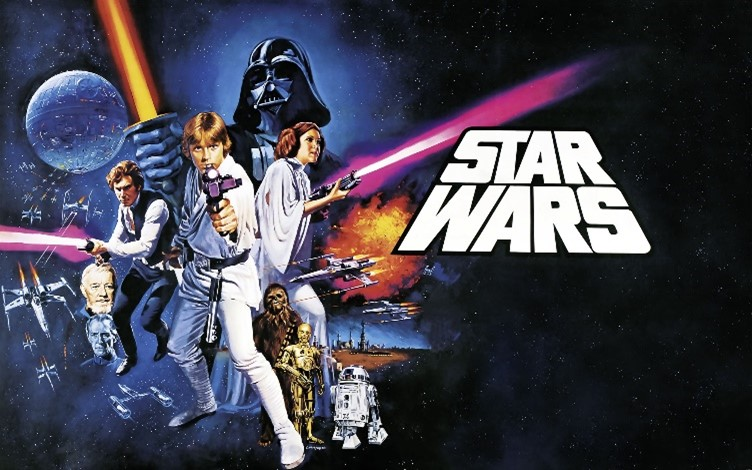
\includegraphics[width=\linewidth]{t2pic.jpg}
\end{wrapfigure}

\par\noindent John Williams often used leitmotifs in his music — recurring musical themes linked to characters or ideas. For example, Darth Vader’s “Imperial March” exudes menace with its pounding brass, while Leia’s Theme evokes grace and longing. These motifs evolve across all the films, reflecting character development and changes in the story.

\vspace{1em}


\par\noindent The soundtrack not only earned Williams an Academy Award but also charted on the Billboard Hot 100 — an incredible achievement for a purely instrumental score. Today, the Star Wars theme is one of the most recognizable pieces of music worldwide, symbolizing heroism, adventure, and the power of cinematic sound.

\par\noindent \vspace{3em}
\begin{tcolorbox}
\noindent\textbf{Mini Whiteboard Questions}
\vspace{1em}

\begin{enumerate}[leftmargin=1em, itemsep=0pt, parsep=0pt, topsep=0pt]
    \item What instruments do you hear?
    \vspace{1em}
    \begin{flushleft}
        Trumpet \hfill Violin \hfill Percussion \hfill Electric guitar    \end{flushleft}
    \vspace{1em}
        \begin{flushleft}
        Flute \hfill Bass guitar \hfill Vocals \hfill Ukulele    \end{flushleft}

        
    \vspace{1em}
    \item Do you like this piece of music?
    \vspace{1em}
    \par \noindent Give reasons why - relating to instruments, tempo and dynamics.
    

      
    \vspace{1em}
\end{enumerate}
\end{tcolorbox}


\newpage

\begin{center}
    \fontsize{18}{22}\selectfont
    \textbf{Task 3 - ‘Flight Of The Bumblebee ’ by Nikolai Andreyevich Rimsky-Korsakov
}
\end{center}

\vspace{1em}

\setlength{\columnsep}{1.5em}
\begin{wrapfigure}{l}{0.3\linewidth}
    \vspace{-0.8em}
    \centering
    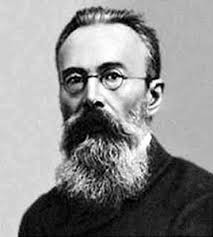
\includegraphics[width=\linewidth]{t3pic.jpg} % Replace with your image
\end{wrapfigure}

\noindent‘Flight of the Bumblebee is an orchestral interlude written by Nikolai Rimsky Korsakov for his opera The Tale of Tsar Saltan, composed in 1899–1900. Its composition is intended to musically evoke the seemingly chaotic and rapidly changing flying pattern of a bumblebee. 


\par \noindent It is not so much the pitch or range of the notes that are played that challenges the musician, but simply the musician's ability to move to them quickly enough. Because of this and its complexity, it requires a great deal of skill to perform.




\vspace{3em}

\begin{tcolorbox}[width=\textwidth]
\noindent\textbf{Mini Whiteboard Questions}

\vspace{1em}

\begin{enumerate}[leftmargin=1em, itemsep=0pt, parsep=0pt, topsep=0pt]
    \item What instruments can you hear playing?
    \vspace{1em}

    \begin{flushleft}
        Piano  \hfill Flute \hfill Violin\hfill Trumpet \\
\vspace{1em}
 Cello  \hfill Tambourine \hfill Glockenspiel\hfill Clarinet \\
        
    \end{flushleft}
    \vspace{1em}
    \item This piece is often seen as a difficult piece to perform. Why do you think this is?
    \vspace{1em}
    
    \item Do you like this piece of music?
    \vspace{1em}
    \par \noindent Give reasons why.
    \vspace{1em}
    


\end{enumerate}
\end{tcolorbox}
\newpage

\begin{center}
    \fontsize{18}{22}\selectfont
    \textbf{Task 4 - ‘In The Hall Of The Mountain King' by Edvard Grieg}
\end{center}
\setlength{\columnsep}{1.5em}
\begin{wrapfigure}{l}{0.3\linewidth}
    \vspace{-0.8em}
    \centering
    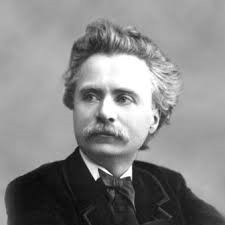
\includegraphics[width=\linewidth]{t4pic.jpg} % Replace with your image
\end{wrapfigure}
\vspace{1em}



\noindent Edvard Grieg was a Norwegian composer and pianist. He is widely considered one of the leading 19th century composers, and his music is part of the standard classical repertoire worldwide. 
\par \noindent His use and development of Norwegian folk music in his own compositions put the music of Norway in the international spotlight.

\par \noindent Grieg's music often evokes the natural landscapes of Norway, using lyrical piano writing and warm orchestration to create a distinct, nationalistic sound that remains popular worldwide today.



\vspace{2em}

\begin{tcolorbox}[width=\textwidth]
\noindent\textbf{Mini Whiteboard Questions}

\vspace{1em}

\begin{enumerate}[leftmargin=1em, itemsep=0pt, parsep=0pt, topsep=0pt]
    \item How would you describe the tempo of this piece at the beginning?
    \vspace{1em}

    \begin{flushleft}
        Slow  \hfill Medium  \hfill Fast \hfill Very fast \\
    \end{flushleft}
    \vspace{1em}
    \item How would you describe the tempo of this piece at the end?
    \vspace{1em}
    \begin{flushleft}
         Slow  \hfill Medium  \hfill Fast \hfill Very fast \\
         \end{flushleft}
    \vspace{2em}
    \item This piece of music has been used on TV before.

\par \noindent    Can you remember what it’s been used on?
    \vspace{2em}
    

\end{enumerate}
\end{tcolorbox}
\newpage

\begin{center}
    \fontsize{18}{22}\selectfont
    \textbf{Task 5 - ‘Radetzky March' by Johann Strauss}
\end{center}
\setlength{\columnsep}{1.5em}
\begin{wrapfigure}{l}{0.3\linewidth}
    \vspace{-0.8em}
    \centering
    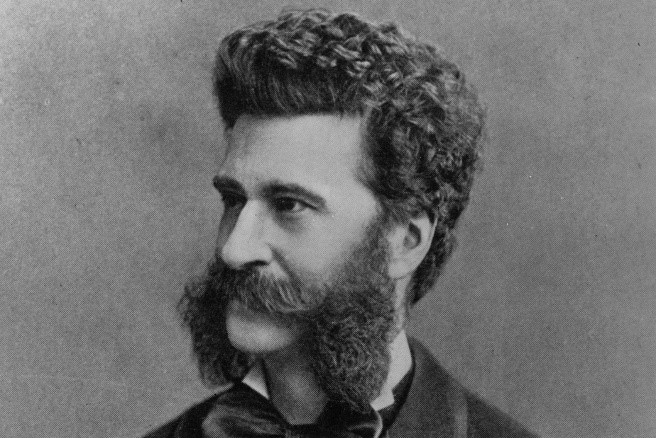
\includegraphics[width=\linewidth]{t5pic.jpg} % Replace with your image
\end{wrapfigure}
\vspace{1em}



\noindent Radetzky March, Op. 228, is a march composed by Johann Strauss.First performed on 31 August 1848 in Vienna, it soon became quite popular among marching soldiers. 

\par \noindent It has been remarked that its tone is more celebratory than martial; Strauss was asked to write the piece to commemorate Radetzky's victory at the Battle of Custoza.
\par \noindent Johann Strauss was an Austrian Romantic composer. He was famous for his waltzes, along with his marching music. 




\vspace{2em}

\begin{tcolorbox}[width=\textwidth]
\noindent\textbf{Mini Whiteboard Questions}

\vspace{1em}

\begin{enumerate}[leftmargin=1em, itemsep=0pt, parsep=0pt, topsep=0pt]
    \item What instruments can you hear playing? 
    \vspace{1em}

    \begin{flushleft}
        Flute  \hfill Guitar  \hfill Violin \hfill Cello \hfill Harp \\
        \vspace{1em}
     Drums  \hfill Vocals  \hfill Bass \hfill Drums \hfill Saxophone \\
    
    \end{flushleft}
    \vspace{1em}
    \item How would you describe the tempo of this song?
    \vspace{2em}
    
    \item What do you think of when you hear this music?


    \vspace{2em}
    

\end{enumerate}
\end{tcolorbox}
\newpage
\begin{landscape}

\begin{center}
    \fontsize{18}{22}\selectfont
    \textbf{New World Symphony Melody}
\end{center}

\vspace{3em}



\begin{center}
    
    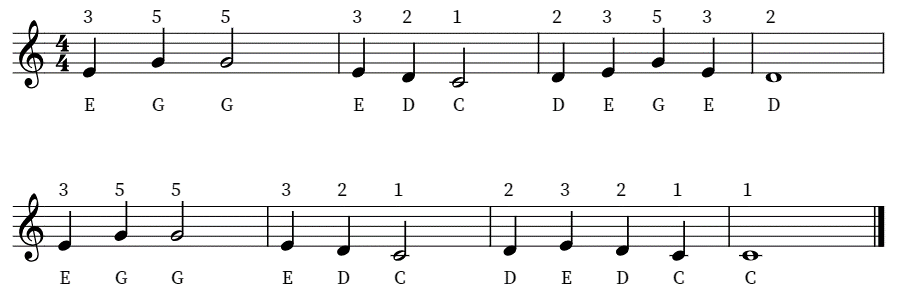
\includegraphics[width=1.4\textwidth]{newworldmelody.png} % Replace with actual image path
\end{center}


    












\newpage
  \begin{center}
    \fontsize{18}{22}\selectfont
    \textbf{New World Symphony Chords}
  \end{center}

  \begin{center}
    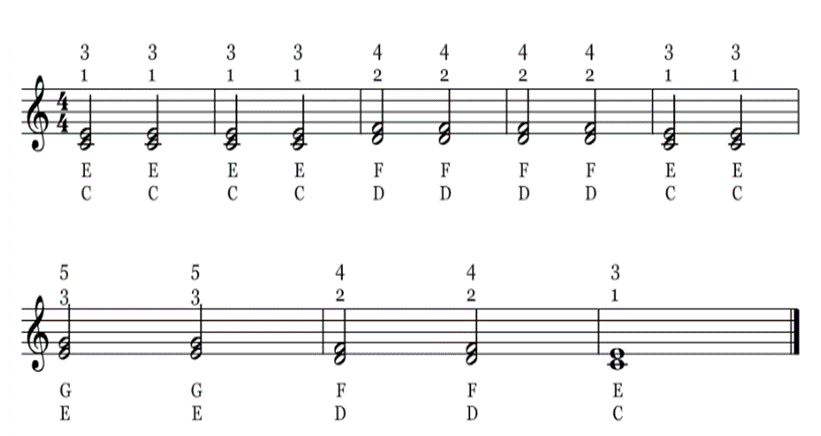
\includegraphics[width=0.9\linewidth, height=0.8\linewidth, keepaspectratio]{newworldchords.png}
  \end{center}



\newpage
  \begin{center}
    \fontsize{18}{22}\selectfont
    \textbf{New World Symphony Melody \& Chords}
  \end{center}

  \begin{center}
    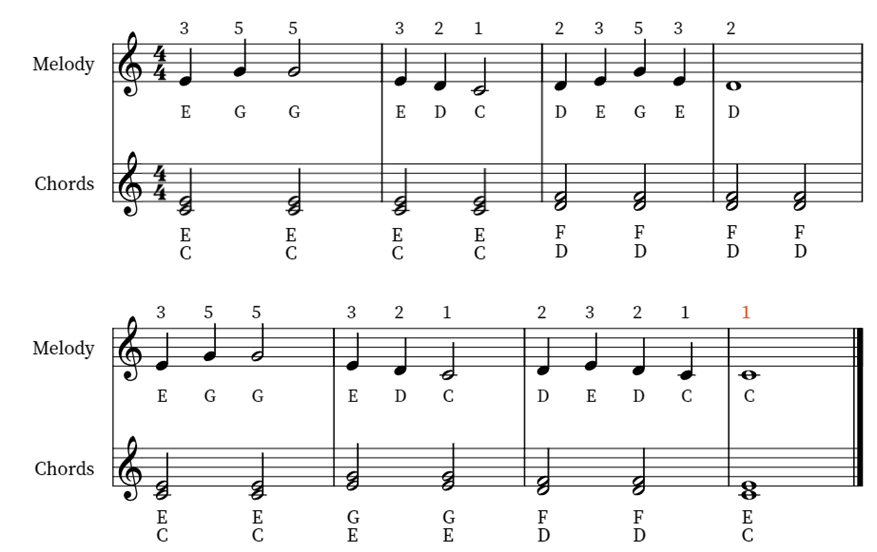
\includegraphics[width=0.9\linewidth, height=0.8\linewidth, keepaspectratio]{newworldscore.png}
  \end{center}


\end{landscape}

\newpage

\begin{center}
    \fontsize{18}{22}\selectfont
    \textbf{Assessment Criteria}
\end{center}

\vspace{1em}

\noindent Your work will be marked according to this table when you are assessed at the end of the half-term.

\vspace{1em}

\begin{center}
\begin{tabularx}{\textwidth}{|c|X|} % Changed to tabularx
\hline
\textbf{Mark} & \textbf{Description} \\
\hline
10 & Can play both extension parts with partner - excellent.\\
\hline
9 & Can play both extension parts with partner - good. \\
\hline
8 & Can play both extension parts. \\
\hline
7 & Can play one extension part. \\
\hline
6 & Plays melody and chords(with partner). \\
\hline
5 & Plays melody and chords (but not with partner). \\
\hline
4 & Plays melody with correct fingers. \\
\hline
3 & Plays melody with correct fingers, possibly unsteady \\
\hline
2 & Plays melody with incorrect fingers, possibly unsteady.\\
\hline
1 & No real work. \\
\hline
\end{tabularx} % Changed to tabularx
\end{center}

\vspace{1em}

\noindent An assessment lesson is an opportunity for you to show your best work, so that you can achieve your highest mark.

\vspace{1em}

\noindent \textbf{How can I achieve my best mark?}

\vspace{1em}

\noindent Before we continue our work, have a look at the table and see what stage you are currently working at.

\noindent For example, if you can only play the melody with correct fingers, then you are currently working at a 4.

\vspace{1em}

\noindent If you are working at a 4, what do you need to do to improve?

\noindent Use this information to help you in your assessment.
\end{document}


